\section{Overview}
\label{sec:overview}

\begin{table} 
%\vspace{-0.15in}
\caption{Objectives of topic-based service discovery.}
%\vspace{-0.1in}
\label{tab:objectives}
\renewcommand{\arraystretch}{1.5}
\renewcommand{\tabcolsep}{0.5em}
\centering
\scriptsize{
\begin{tabular} {p{1cm}p{5cm}}
\toprule
\textbf{Objective} & \textbf{Description} \\
\hline
G1 & Max-min fair allocation of topic table across topics \\
\hline
%G1 & Regardless of the topic they are registering, advertisers should not be globally denied from registering their ad. \\
%\hline
G2 & All advertisers within each topic should have a similar probability of being discovered. \\
\hline
G3 & The load (in terms of messaging overhead) should be equally distributed across registrars. \\
\hline
G4 & The registration operations should be efficient in terms of time. \\
\hline
G5 & The registration operations should be efficient in terms of messaging, computational, and state maintenance overhead. \\
\hline 
G6 & The search operation should be efficient in terms of time and messages sent to nodes (hop count) for all the topics independent of their popularity. \\
\hline
%G7 & The number of registrations should be sufficient for an efficient discovery. \\ Onur: I don't think we need this
%\hline
G7 & The protocol should be resistant to network dynamics (nodes joining and leaving). \\
\hline 
G8 & The protocol should be resistant to attacks by malicious nodes or their Sybils. \\
\hline
\end{tabular}
}
\vspace{-0.2in}
\end{table}


The end-goal of service discovery is to enable nodes to be discovered under topics which they choose to be associated with in a secure, robust and efficient manner. \Cref{tab:objectives} provides a comprehensive list of the design objectives, which we refer to in the text below. We define two main questions which need to be answered before achieving our goals:
\begin{enumerate}
    \item Where should specific ads be placed in the network?
    \item How to ensure fairness with limited resources of the registrars in an open system with malicious nodes?
\end{enumerate}

\para{Where should specific ads be placed in the network?} We envision a large number of topics in the system. However, it is difficult to predict the actual number. The number of topics in the system might also change over time. 

The Ethereum DHT offers the default \emph{put} and \emph{get} operations that store data on a single node who's ID is the closest to the hash of the data. The procedures uniformly distribute the topics across the network and make efficient use of the existing routing in the DHT table (\textbf{+G4, +G5}). Unfortunately, such an approach results in unequal load across registrar if the popularity of the topics vary significantly. Advertisers storing popular topics would receive a large portions of the request (\textbf{-G3}). Furthermore, when a topic-specific registrar leaves the network, the registration process must re-start from scratch causing disturbance in the network (\textbf{-G7}). It is also fairly easy for an attacker to generate Sybil nodes with IDs close to the topic hash and take control over the entire topic-specific traffic (\textbf{-G8}). Multiple work  proposed to enhance regular \emph{put} and \emph{get} operations by simultaneously using multiple hash functions [\hl{REF}] or increasing the number of nodes storing values for each key[\hl{REF}]. Unfortunately, such approaches only slightly increase the amount of resources a malicious player needs to launch a successful attack against a topic. 

Alternatively, advertisers could place their ads on random advertisers across the entire network. This approach is much more difficult to attack as a malicious player would need to take control over the entire network to control a single topic (\textbf{+G8}). Furthermore, random placement is resistance to network dynamics, as registrations are stored on multiple registrars (\textbf{+G7}). It also achieves good load balance across registrars regardless of the topic popularity distribution (\textbf{+G3}). On the other hand, random placement makes it difficult for searchers to find placed placed ads, especially for unpopular topic. Either, the advertisers place a large number of ads to simplify the search, or searchers need to consult multiple registrars before finding a relevant ad and simplify the registration. Both approaches require significant amounts of time ((\textbf{-G3}) and additional traffic (\textbf{-G4}). 

\sysname implements an alternative approach that combines advantages of both the regular DHT \emph{put}, \emph{get} operations and the random placements. When an advertiser wants to place an ad for a topic, it first hashes the topic and creates a topic-specific \textbf{Topic Table} (\Cref{fig:ticket_table}. The topic table is similar to the DHT routing table but pre-populated with peers from the routing table but organized in buckets in a different way. It creates buckets based on the distance from the topic hash instead of relying on the distance from the node ID (as the DHT routing table does). To advertiser starts by a topic table bucket that is the furthest away from the topic hash (\ie \emph{bucket 1} on \Cref{fig:ticket_table}) and randomly chooses a fixed amount of peers from this bucket where the advertiser will attempt to register. It will then move to the next bucket (\ie \emph{bucket 1} on \Cref{fig:ticket_table}) and repeats the operation gradually moving towards the topic hash. The search operation closely mimics the registration but stops when enough ads are found. 

Combining topic-oriented bucket organization together with intra-bucket random ad placement makes the system secure and efficient at the same time. Each registration operation generates a fixed amount of traffic regardless of the topic popularity (\textbf{+G5}). Search operations for highly popular topic, can stop after consulting just a few buckets if enough peers are found. It speeds up the process (\textbf{+G4}), lowers the system message overhead (\textbf{+G5}) and prevents searchers from consulting advertisers close to the topic hash ensuring good load balance (\textbf{+G3}). At the same time, searchers of low-popularity topics are guaranteed to find ads by eventually reaching the closest bucket in a bounded amount of steps. \sysname is secure against Sybil attacks (\textbf{+G8}) and resistant against node failures (\textbf{+G7}). Failure or corruption of a single node (or a group of nodes) close to the topic hash does not prevent honest nodes from discovering their honest peers. Furthermore, attacking every advertiser holding topic-specific ads is impossible due to the unpredictable nature of placing ads. 


\begin{figure}
    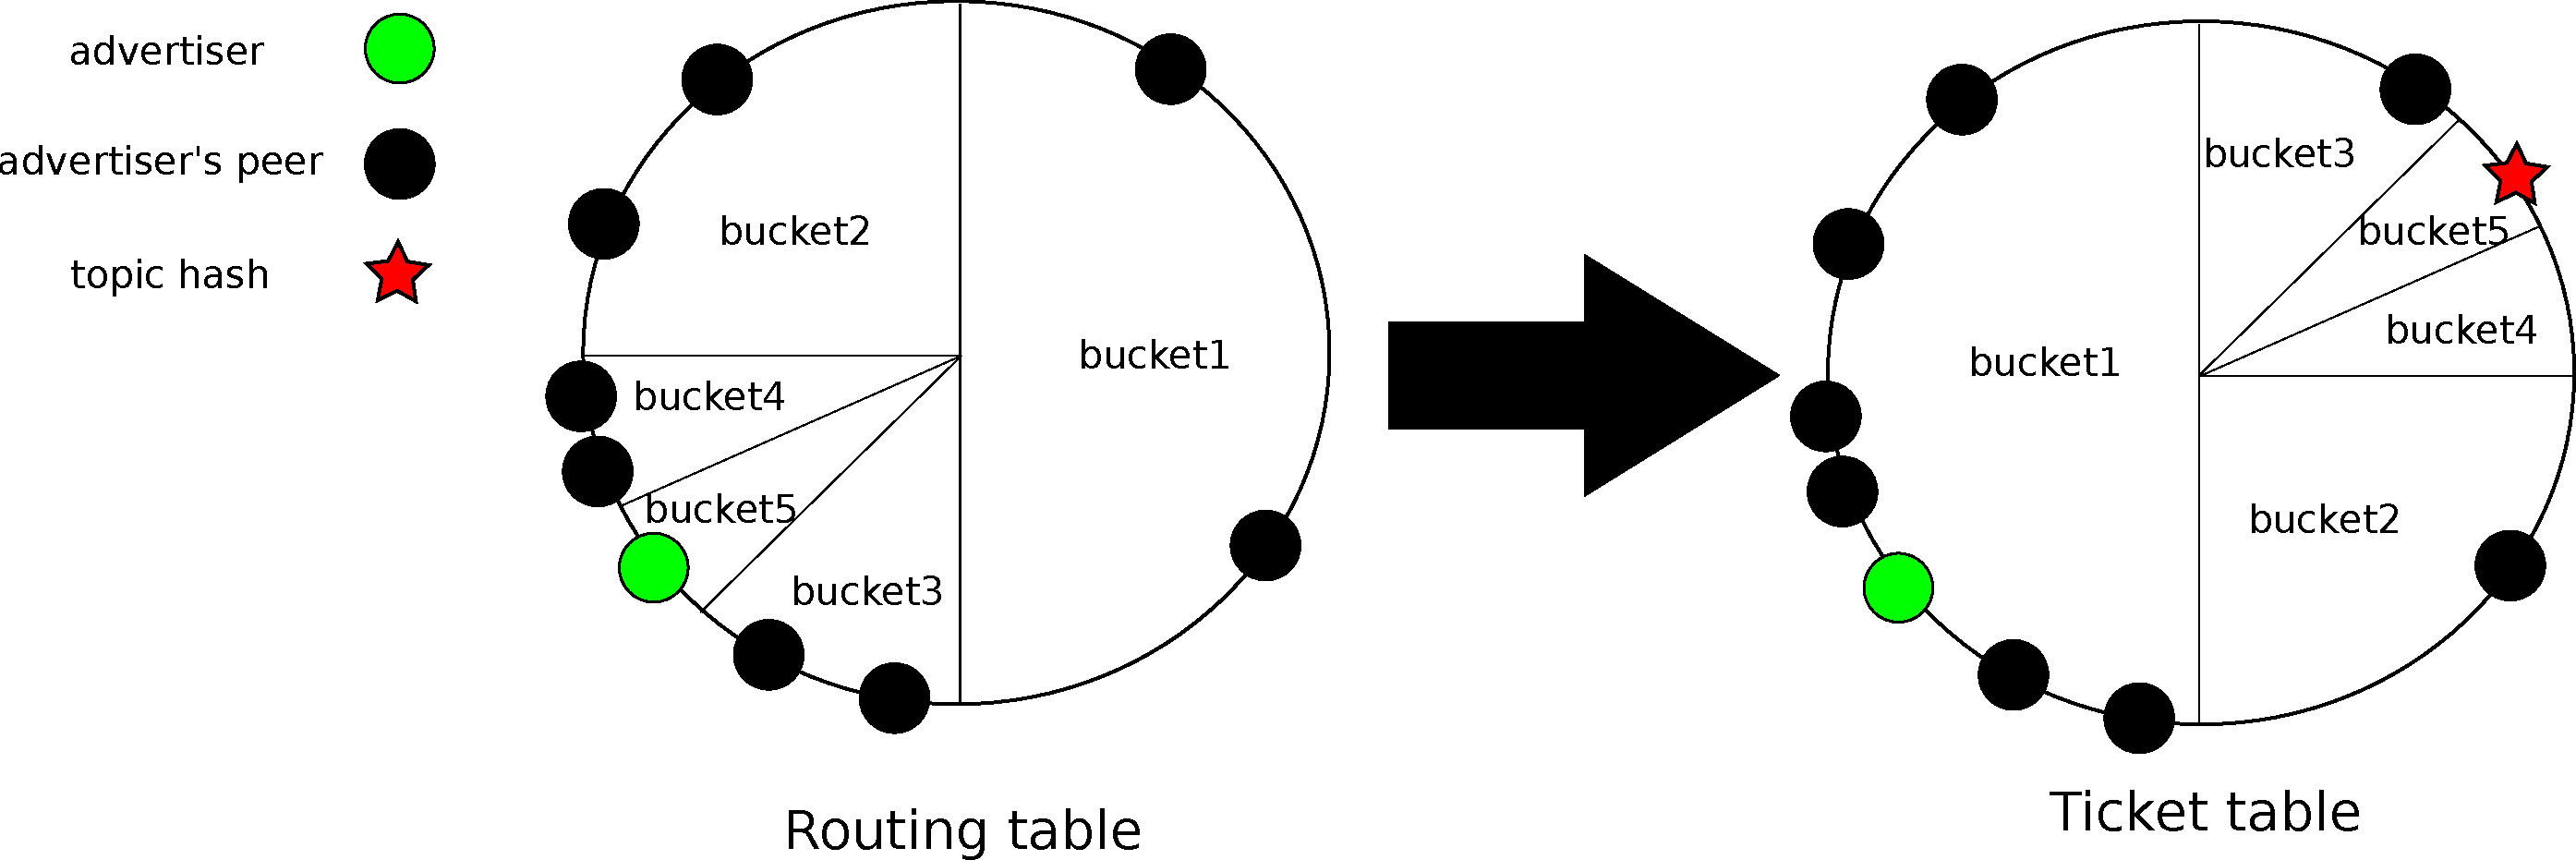
\includegraphics[width=0.45\textwidth]{img/ticket_table}
    \caption{Creation of ticket table from the routing table.}
    \label{fig:ticket_table}
 \end{figure}
 
 \para{How to ensure fairness with limited resources of the registrars in an open system with malicious nodes?} We assume the registrars will store ads in a fixed size \textbf{topic table}. The ad distribution procedure from above attempts to spread the load equally across nodes in the network. However, malicious nodes may decide to ignore the protocol trying to overload one or multiple registrars with their traffic. Furthermore, honest advertisers registering for large number of topics may exhaust limited resources of the registrars. 
 
 \sysname solves this problems by using a lightweight \textit{waiting-time-based admission mechanism}. When an advertisers sends an ad placement request to a registrar, the registrar will calculate an amount of time the advertisers needs to wait before being admitted (\ie the waiting time). The registrar also issues a \textbf{ticket} to the advertiser. The ticket specifies the time of the initial request, the calculated waiting time and is digitally signed by the registrar. The advertiser includes the ticket in its following registration requests and will be admitted only if the waiting is lower than the time the advertiser already waited for (as indicated by the initial request time). 
 
 The waiting time is calculated based on the diversity of the request (\ie how different is the request from ads already in the topic table?) and space left in the topic table. The more different the request is (in terms of the IP/ID of the registrar and the topic) from the current content of the topic table, the lower the calculated waiting time. At the same time, the calculated waiting time increases as the topic table fill in. The diversity score simplifies the admission for unpopular topic, as receive lower waiting times and are more likely to be admitted (\textbf{+G1, +G2}). Furthermore, high diversity of the topic table makes \sysname resistant to network dynamics (\textbf{+G7}). The proposed admission mechanism also prevents Sybil attacks performed by an attacker with a limited amount of resources (\textbf{+G8}). For instance, consecutive registration attempts from a single IP address will receive increasing waiting time eventually blocking further registration attempts made by the attacker. Including the current topic table size in the waiting time improves the load distribution. Registrars located close to the hashes popular topics will quickly will their topic table and return higher waiting times to the advertiser limiting the incoming traffic (\textbf{+G3}). 